\subsection{Le besoin de la communauté}

Pour que le projet soit un succès, il est nécessaire de répondre à certains besoins de la future communauté. Le psychologue Abraham Maslow a développé en 1940 une théorie concernant la motivation des individus et il affirme que chaque action est motivé selon un besoin bien particulier.
Dans sa théorie, Maslow réparti les différents besoins en cinq catégorie :
\begin{itemize}
	\item besoin physiologique (faim, soif, respiration, reproduction...)
	\item besoin de sécurité (recherche d'un environnement stable)
	\item besoin d'appartenance et d'amour
	\item besoin d'estime (confiance en soi, reconnaissance et appréciation)
	\item besoin d'accomplissement
\end{itemize}

Ces besoins sont réparti selon le diagramme suivant, en couche successive par ordre d'importance. Pour que l'impact soit fort, il est nécessaire de toucher le futur candidat sur une ou plusieurs de ces catégorie afin de susciter chez lui une envie de rejoindre le département ASI

\begin{center}
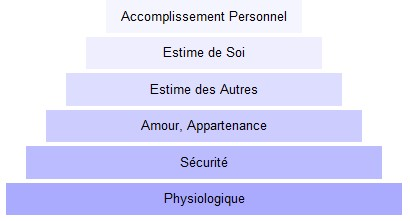
\includegraphics[scale=0.5]{./image/pyramidemaslow.jpg}
\end{center}
~~\\
\indent Le but de notre projet est de donnée une meilleure visibilité au département ASI afin de donner envie aux potentiels candidats de postuler. Clairement, les deux premières catégories ne font pas partie des besoins que la présence du département ASI sur les réseaux sociaux peut satisfaire (même si la formation permet de "mettre du beurre dans les épinards"). ~~\\
\indent En revanche les trois dernières sont beaucoup plus à portée. 
\indent De part l'ambiance "école" de l'INSA de Rouen, et des diverses rencontres du groupe INSA plus généralement, le futur postulant va souhaiter intégrer le département et ainsi faire partie du groupe. ~~\\
\indent Le département ASI, même si moins bien coté que le département IF de l'INSA de Lyon reste une formation d'excellence et prestigieuse. Cette reconnaissance est tout à fait à même de satisfaire le besoin d'estime du futur postulant. ~~\\
\indent Enfin, le besoin d'accomplissement est certainement l'axe majeur de la formation d'ingénieur ASI dans la mesure où celui-ci sera amené, lors de la formation, comme durant toute sa carrière professionnelle de développer et mettre en place des projets de grande envergure.

\subsection{Faire revenir un utilisateur}

